\documentclass[a4paper,11pt,exos]{nsi} % COMPILE WITH DRAFT


\pagestyle{empty}
\begin{document}

%Exercice 1E11-2



\classe{\premiere spé}
\titre{Ceinture orange 01 - Corrigé}
\maketitle

\begin{exercice}[ : Résoudre une inéquation du second degré]
    Résoudre dans $\R$ les inéquations suivantes :
    \begin{multicols}{2}
        \begin{enumerate}
            \item $-5x^2+10x-8\geqslant 0$
            \item $-2x^2-4x+16\geqslant 0$
	        %\item $-x^2-2x-3\leq 0$
        \end{enumerate}
    \end{multicols}
    
\end{exercice}

\begin{enumerate}
    \item Soit $P$ le polynôme défini pour tout $x$ de $\mathbb R$ par $P(x)=-5x^2+10x-8$.\\On cherche à résoudre $P(x)\geqslant 0$.\\Pour cela, on cherche ses racines éventuelles.\\$\Delta = 10^2-4\times(-5)\times(-8)=-60$\\$\Delta<0$ donc le polynôme $P$ n'admet pas de racine.\\ Il est toujours du signe de $a=-5<0$, donc $P(x)<0$ pour tout $x$ de $\mathbb{R}$.\\ On en déduit $S=\emptyset$.
    \item Soit $P$ le polynôme défini pour tout $x$ de $\mathbb R$ par $P(x)=-2x^2-4x+16$.\\On cherche à résoudre $P(x)\geqslant 0$.\\Pour cela, on cherche ses racines éventuelles.\\$\Delta = (-4)^2-4\times(-2)\times16=144$\\$\Delta>0$ donc  le polynôme admet deux racines : $x_1 = \dfrac{-b-\sqrt{\Delta}}{2a}$ et $x_2 = \dfrac{-b+\sqrt{\Delta}}{2a}$.\\$x_1 =\dfrac{4-\sqrt{144}}{-4}=2$\\$x_2 =\dfrac{4+\sqrt{144}}{-4}=-4$\\On sait qu'un polynôme du second degré est du signe de $a$ à l'extérieur de ses racines.\\Comme $a=-2<0$, on peut dire que $P(x)\geq 0$ sur $S=]-\infty;-4]\cup[2;+\infty[$\\On peut résumer le signe du polynôme dans un tableau de signes :\\
    \begin{tikzpicture}[baseline, scale=0.5]
        \tkzTabInit[lgt=8,deltacl=0.8,espcl=5]{ $x$ / 2, $-2x^2-4x+16$ / 2}{ $-\infty$, $-4$, $2$, $+\infty$}
        \tkzTabLine{  , -, z, +, z, -}
        \end{tikzpicture}
    \\ Finalement $S=[-4;2]$.
%\item Soit $P$ le polynôme défini pour tout $x$ de $\mathbb R$ par $P(x)=-x^2-2x-3$.\\On cherche à résoudre $P(x)\leq 0$.\\Pour cela, on cherche ses racines éventuelles.\\$\Delta = (-2)^2-4\times(-1)\times(-3)=-8$\\$\Delta<0$ donc le polynôme $P$ n'admet pas de racine.\\ Il est toujours du signe de $a=-1<0$, donc $P(x)<0$ pour tout $x$ de $\mathbb{R}$.\\ On en déduit $S=\mathbb{R}$.
\end{enumerate}


\end{document}